\documentclass[dvipdfmx]{jsarticle}
\usepackage{amsmath}
\usepackage{amssymb}
\usepackage{enumitem}
\usepackage{tikz}
\usepackage{pgfplots}

\pgfplotsset{compat=1.18}
\usepgfplotslibrary{fillbetween}
\usetikzlibrary{patterns}
\usetikzlibrary{calc}
\usetikzlibrary{perspective}

\setlist[enumerate,1]{label=\huge\arabic*.}

\begin{document}
\begin{enumerate}
    \item 座標平面上の曲線$C:y=x^3-x$の接線のうち、点$P(a, b)$を通るものがちょうど3本存在するような点$(a,b)$の存在範囲を図示するとき、その境界線の方程式を求めよ。\\
    \\
    接点の$x$座標を$t$とする。
    与えられた曲線の方程式より、
    \[y'=3x^2-1\]
    なので、接線の方程式は
    \[y=(3t^2-1)(x-t)+t^3-t\quad\Longleftrightarrow\quad y=(3t^2-1)x-2t^3\]
    これが$(a,b)$を通るので、
    \begin{gather*}
        b=(3t^2-1)\cdot a-2t^3\\
        2t^3-3at^2+a+b=0
    \end{gather*}
    題意の条件が成り立つのは、この$t$に関する3次方程式の実数解が3つ存在するとき、すなわち$f(t)=2t^3-3at^2+a+b$としたときに、$y=f(t)$と$y=0$との共有点が3つになるときである。
    \begin{align*}
        f'(t)&=6t^2-6at\\
             &=6t(t-a)
    \end{align*}
    である。
    \begin{enumerate}[label=(\roman*)]
        \item $a>0$のとき、増減表は下図となる。\\
        \[\begin{array}{c||c|c|c|c|c}
            t     & \cdots   & 0   & \cdots   & a        & \cdots   \\
            \hline
            f'(t) & +        & 0   & -        & 0        & +        \\
            \hline
            f(t)  & \nearrow & a+b & \searrow & -a^3+a+b & \nearrow
        \end{array}\]
        よって、$y=f(t)$と$y=0$との共有点が3つになるのは、$a+b>0$かつ$-a^3+a+b<0$、すなわち$b>-a$かつ$b<a^3-a$のとき。
        \item $a=0$のとき、$f'(t)=6t^2\geq0$なので、$f(t)$は増加関数であり、$y=f(t)$と$y=0$との共有点が3つになることはない。
        \item $a<0$のとき、増減表は下図となる。\\
        \[\begin{array}{c||c|c|c|c|c}
            t     & \cdots   & a        & \cdots   & 0   & \cdots   \\
            \hline
            f'(t) & +        & 0        & -        & 0   & +        \\
            \hline
            f(t)  & \nearrow & -a^3+a+b & \searrow & a+b & \nearrow
        \end{array}\]
        よって、$y=f(t)$と$y=0$との共有点が3つになるのは、$-a^3+a+b>0$かつ$a+b<0$、すなわち$b>a^3-a$かつ$b<-a$のとき。
    \end{enumerate}
    (i)~(iii)より、点(a,b)の存在範囲は下図。
    \begin{center}\begin{tikzpicture}
        \begin{axis}[
            axis lines = middle,
            axis on top,
            xlabel = $a$,
            ylabel = $b$,
            xmin = -2.5, xmax = 2.5,
            ymin = -3, ymax = 3,
            samples = 100,
            domain = -2:2,
            xtick = \empty,
            ytick = \empty,
        ]
        \addplot [name path=C, thick] {x^3 - x};
        \node at (axis cs:0.9,2.2) {$b=a^3-a$};
        \addplot [name path=L, thick] {-x} node[below] {$b=-a$};
        \addplot [gray] fill between [of=C and L];
        \filldraw [fill=white, draw=black, thick] (axis cs:0,0) circle (2pt);
        \node at (axis cs:0,0) [below left] {$O$};
        \node at (axis cs:-1.5,2.3) {(境界は含まない)};
        \end{axis}
    \end{tikzpicture}\end{center}
    よって、求める境界線の方程式は、$b=a^3-a$と$b=-a$。
    \vspace{3cm}
    \item $n$を2以上の自然数とする。$n^4+4$が素数となるような$n$をすべて求めよ。\\
    \\
    法を5とする。\\
    \begin{enumerate}[label=(\roman*)]
        \item $n\equiv\pm1$のとき\\
        $n^2\equiv1$より、
        \[n^4+4\equiv1^2+4\equiv0\]
        よって、$n^4+4$が素数となるのは$n^4+4=5$のときのみであり、このとき$n=1$。しかしこれは、$n$が2以上の自然数であることに反する。よって、題意を満たす$n$は存在しない。
        \item $n\equiv\pm2$のとき\\
        $n^2\equiv4$より、
        \[n^4+4\equiv4^2+4\equiv0\]
        よって、(i)と同様にして、題意を満たす$n$は存在しない。
        \item $n\equiv0$のとき\\
        $n=5N$($N$は自然数)とおける。このとき、
        \begin{align*}
            n^4+4&=(5N)^4+4\\
                 &=\left((5N)^2\right)^2+2^2\\
                 &=(25N^2+2)^2-2\cdot(5N)^2\cdot2\\
                 &=(25N^2+2)^2-(10N)^2\\
                 &=(25N^2+10N+2)(25N^2-10N+2)\\
        \end{align*}
        ここで、
        \[25N^2-10N+2=25\left(N-\frac{1}{5}\right)^2+1\geq17\quad(\because N\geq1)\]
        であり、$N>0$より$25N^2+10N+2>25N^2-10N+2$なので、$n^4+4$は必ず合成数となる。よって、$n^4+4$が素数となるような$n$は存在しない。
    \end{enumerate}
    (i)~(iii)より、題意を満たす$n$は存在しない。
    \vspace{3cm}
    \item 複素数平面上で、点$z$が原点を中心とする半径1の円周上を動くとき、$w=z+\frac{2}{z}$が描く図形は何か。\\
    \\
    点$z$は原点を中心とする半径1の円周上を動くので、$z=\cos\theta+i\sin\theta\ (0\leq\theta<2\pi)$とおける。このとき、
    \begin{align*}
        w&=z+\frac{2}{z}\\
         &=\cos\theta+i\sin\theta+2\cdot(\cos\theta+i\sin\theta)^{-1}\\
         &=\cos\theta+i\sin\theta+2\cdot(\cos\theta-i\sin\theta)\\
         &=3\cos\theta-i\sin\theta
    \end{align*}
    よって、$w$は長軸6、短軸2の楕円を描く。
    \vspace{3cm}
    \item 積分$I=\int_0^\pi e^{-x}\sin xdx$の値を求めよ。\\
    \\
    \begin{align*}
        I&=\left[-e^{-x}\sin x\right]_0^\pi-\int_0^\pi (-e^{-x}\cos x)dx\\
         &=0-\left(\left[e^{-x}\cos x\right]_0^\pi-\int_0^\pi e^{-x}(-\sin x)dx\right)\\
         &=-\left(e^{-\pi}\cdot(-1)-1\cdot1\right)-I\\
         &=1+e^{-\pi}-I
    \end{align*}
    よって、
    \begin{align*}
        2I&=1+e^{-\pi}\\
         I&=\frac{1+e^{-\pi}}{2}
    \end{align*}
    \vspace{3cm}
    \item 三角形ABCにおいて、辺ABを$2:1$に内分する点をD、辺ACを$3:2$に内分する点をEとする。線分BEとCDの交点をPとし、直線APと辺BCの交点をFとする。このとき、比$\text{BF}:\text{FC}$を求めよ。\\
    \\
    \begin{center}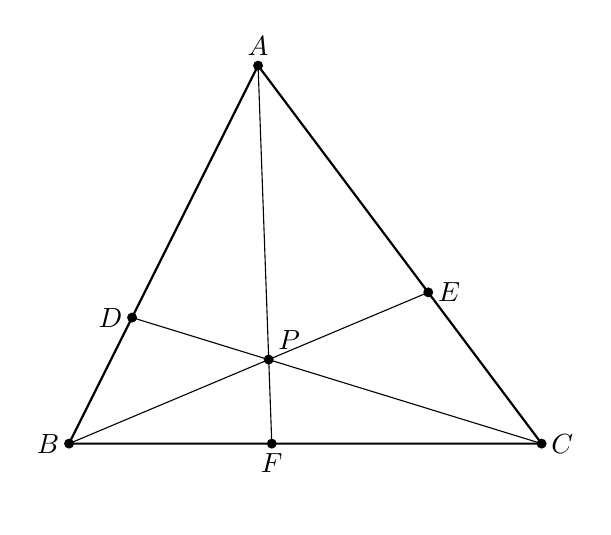
\begin{tikzpicture}[scale=1.2]
        \coordinate (A) at (2, 4);
        \coordinate (B) at (0, 0);
        \coordinate (C) at (5, 0);

        \coordinate (D) at ($(A)!2/3!(B)$);
        \coordinate (E) at ($(A)!3/5!(C)$);

        \draw[name path=BE] (B) -- (E);
        \draw[name path=CD] (C) -- (D);
        \path[name intersections={of=BE and CD, by=P}];

        \path[name path=AP_line] (A) -- ($(A)!1.5!(P)$);
        \path[name path=BC] (B) -- (C);
        \path[name intersections={of=AP_line and BC, by=F}];

        \draw[thick] (A) -- (B) -- (C) -- cycle;
        \draw (A) -- (F);

        \foreach \p/\pos in {A/above, B/left, C/right, D/left, E/right, P/above right, F/below} {
            \fill (\p) circle (1.5pt);
            \node[\pos] at (\p) {$\p$};
        }
    \end{tikzpicture}\end{center}
    チェバの定理より、
    \begin{gather*}
        \frac{\text{AD}}{\text{DB}}\cdot\frac{\text{BF}}{\text{FC}}\cdot\frac{\text{CE}}{\text{EA}}=1\\
        \frac{2}{1}\cdot\frac{\text{BF}}{\text{FC}}\cdot\frac{2}{3}=1\\
        \frac{\text{BF}}{\text{FC}}=\frac{3}{4}
    \end{gather*}
    よって、$\text{BF}:\text{FC}=3:4$
    \vspace{3cm}
    \item サイコロを$n$回投げて、出た目の積を$X_n$とする。$X_n$が5で割り切れる確率$p_n$を求めよ。\\
    \\
    求める確率は一度も5が出ない確率なので、
    \[p_n=1-\left(\frac{5}{6}\right)^n\]
    \vspace{3cm}
    \item 実数$x,\ y$が$x^2+xy+y^2=3$を満たすとき、$x+y$の取りうる値の最大値を求めよ。\\
    \\
    $x+y=u,\ xy=v$とする。与式より、
    \begin{gather*}
        (x+y)^2-xy=3\\
        u^2-v=3\\
        v=u^2-3
    \end{gather*}
    また、解と係数の関係より、$x$と$y$は$t$に関する二次方程式$t^2-ut+v=0$の2解である。$x$と$y$が実数であるのは、この方程式の判別式を$D$としたときに$D\geq0$のときである。
    \[D=u^2-4v\]
    より、
    \[u^2-4v\geq0\]
    これらより、
    \begin{gather*}
        u^2-4(u^2-3)\geq0\\
        3u^2\leq12\\
        u^2\leq4\\
        -2\leq u\leq2
    \end{gather*}
    よって、求める最大値は2。
    \vspace{3cm}
    \item 極限値$\lim_{n\to\infty}\frac{1}{n}\sum_{k=1}^n\log\left(1+\frac{k}{n}\right)$を求めよ。\\
    \\
    \begin{align*}
         &\lim_{n\to\infty}\frac{1}{n}\sum_{k=1}^n\log\left(1+\frac{k}{n}\right)\\
        =&\int_0^1\log(1+x)dx=\left[(1+x)\log(1+x)-(1+x)\right]_0^1\\
        =&\left(2\log2-2\right)-\left(1\cdot0-1\right)\\
        =&2\log2-1
    \end{align*}
    \vspace{3cm}
    \item 四面体OABCにおいて、$\text{OA}=\text{OB}=\text{OC}=1$、$\angle AOB=\angle BOC=\angle COA=90^\circ$とする。頂点Oから底面ABCに下した垂線の足をHとするとき、OHの長さはいくらか。\\
    \\
    \begin{center}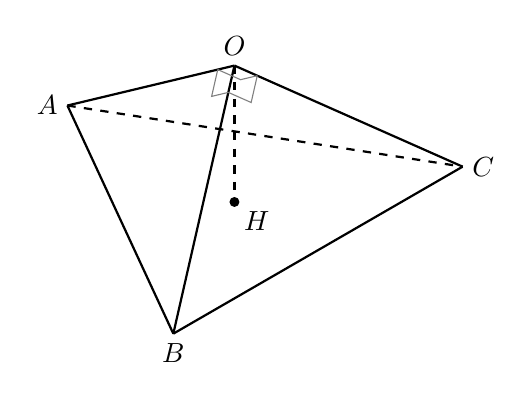
\begin{tikzpicture}[
        scale=3, 
        x={(-0.866cm, -0.5cm)}, 
        y={(0.866cm, -0.5cm)}, 
        z={(0cm, 1cm)},
        >=stealth
    ]
        \coordinate (H) at (0, 0, 0);
        
        \pgfmathsetmacro{\R}{sqrt(6)/3}
        \coordinate (A) at (0, -\R, 0);
        \coordinate (B) at ({\R*cos(30)}, {\R*sin(30)}, 0);
        \coordinate (C) at ({\R*cos(150)}, {\R*sin(150)}, 0);

        \pgfmathsetmacro{\h}{sqrt(3)/3}
        \coordinate (O) at (0, 0, \h);

        % \fill[orange!10, opacity=0.7] (A) -- (B) -- (C) -- cycle;
        
        \draw[thick] (B) -- (C);
        
        \draw[dashed, very thick] (O) -- (H);
        \fill (H) circle (0.6pt);

        \draw[thick] (A) -- (B);
        \draw[thick, dashed] (A) -- (C);
        \draw[thick] (O) -- (A);
        \draw[thick] (O) -- (B);
        \draw[thick] (O) -- (C);

        \begin{scope}[gray, thin]
            \draw ($(O)!0.1!(A)$) -- ($(O)!0.1!(A)+(O)!0.1!(B)-(O)$) -- ($(O)!0.1!(B)$);
            \draw ($(O)!0.1!(B)$) -- ($(O)!0.1!(B)+(O)!0.1!(C)-(O)$) -- ($(O)!0.1!(C)$);
            \draw ($(O)!0.1!(C)$) -- ($(O)!0.1!(C)+(O)!0.1!(A)-(O)$) -- ($(O)!0.1!(A)$);
        \end{scope}

        \node[above] at (O) {$O$};
        \node[left] at (A) {$A$};
        \node[below] at (B) {$B$};
        \node[right] at (C) {$C$};
        \node[below right] at (H) {$H$};

    \end{tikzpicture}\end{center}
    三角錐OABCの体積は
    \[\frac{1}{3}\cdot\left(\frac{1}{2}\cdot1\cdot1\right)\cdot1=\frac{1}{6}\]
    一方、ヘロンの公式より、$s=\frac{\text{AB}+\text{BC}+\text{CA}}{2}=\frac{3\sqrt{2}}{2}$とすると、
    \[\triangle\text{ABC}=\sqrt{s(s-\text{AB})(s-\text{BC})(s-\text{CA})}=\sqrt{\frac{3\sqrt{2}}{2}\cdot\left(\frac{\sqrt{2}}{2}\right)^3}=\frac{\sqrt{3}}{2}\]
    よって、
    \begin{gather*}
        \text{三角錐OABC}=\frac{1}{3}\cdot\triangle\text{ABC}\cdot\text{OH}\\
        \text{OH}=\frac{1}{6}\cdot3\cdot\frac{2}{\sqrt{3}}=\frac{1}{\sqrt{3}}=\frac{\sqrt{3}}{3}
    \end{gather*}
    \vspace{3cm}

    \item $f(x)=|x^2-1|$とする。方程式$f(x)=kx+2$が異なる4つの実数解をもつような定数$k$の範囲を求めよ。\\
    \\
    $f(x)=kx+2$が異なる4つの実数解をもつのは、$y=f(x)$と$y=kx+2$のグラフが異なる4点で交わるときである。$y=f(x)$のグラフは下図となる。
    \begin{center}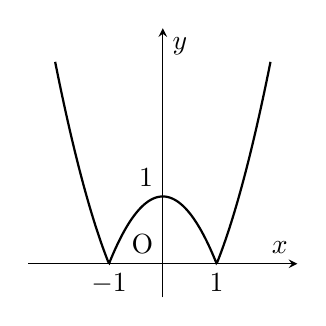
\begin{tikzpicture}
        \begin{axis}[
            axis lines = middle,
            xlabel = $x$,
            ylabel = $y$,
            domain = -2:2,
            samples = 200, % グラフを滑らかにするために多めに設定
            ymin = -0.5, ymax = 3.5,
            xmin = -2.5, xmax = 2.5,
            width = 5cm, height = 5cm,
            xtick = \empty, ytick = \empty,
        ]
            % y = |x^2 - 1| の描画
            \addplot[thick] {abs(x^2 - 1)};

            % 頂点や交点のプロット(任意)
            \node[above left] at (axis cs:0,0) {O};
            \node[above left] at (axis cs:0,1) {$1$};
            \node[below] at (axis cs:1,0) {$1$};
            \node[below] at (axis cs:-1,0) {$-1$};
        \end{axis}
    \end{tikzpicture}\end{center}
    $y=f(x)$と$y=kx+2$のグラフの$x\leq-1,\ 1\leq x$の部分の共有点の個数は、
    \[\begin{cases}
        -2\leq k\leq 2のとき\quad2個\\
        k<-2,\ 2<kのとき\quad1個
    \end{cases}\]
    また、$-x^2+1=kx+2\Leftrightarrow x^2+kx+1=0$の判別式を$D$とすると、
    \[D=k^2-4\]
    なので、$-x^2+1=0$と$kx+2=0$は、$k=\pm2$のとき$x=\mp1$で接する。
    よって、$y=f(x)$と$y=kx+2$のグラフの$-1<x<1$の部分の共有点の個数は、
    \[\begin{cases}
        -2\leq k\leq 2のとき\quad0個\\
        k<-2,\ 2<kのとき\quad1個
    \end{cases}\]
    以上より、$y=f(x)$と$y=kx+2$のグラフの共有点の個数は、任意の$k$に対して2個となる。
    よって、題意を満たす$k$は存在しない。
\end{enumerate}
\end{document}